\documentclass[compress,violet,10pt]{beamer}

\mode<presentation>
\usetheme{Warsaw}

\usepackage{multicol}
\usepackage{amsmath}
\usepackage{caption}
\usepackage{amssymb}
\usepackage{multirow}
\usepackage[numbers]{natbib}
\usepackage{framed}
\usepackage{booktabs}
\usepackage{amsfonts}
\usepackage{hyperref}
\usepackage{graphics} % for including figures
\usepackage{graphicx} % for including figures
\usepackage[update,prepend]{epstopdf} % for including eps in pdf
\def\pdfshellescape{1} % for auto converting eps to pdf
\graphicspath{{../img/}}

\newcommand*\rfrac[2]{{}^{#1}\!/_{#2}}
\newcommand{\traindata}{\ensuremath{\mathcal{T}}}
\newcommand{\matD}{\ensuremath{\mathrm{D}} }

\useoutertheme[subsection=false]{smoothbars}
\setbeamertemplate{caption}[numbered]
\setbeamercovered{transparent}

\title{Domain Driven Decompositional Semantics}

\author[Pranjal Singh]
{\textbf{Pranjal Singh}\\ {\small Supervisor: Dr. Amitabha Mukerjee}}
\date{June 15, 2015}

\institute{\vspace{2mm} 
B.Tech - M.Tech Dual Degree\\
\vspace{.2cm}Thesis Defense\\
\vspace{.2cm}Department of Computer Science \& Engineering\\ IIT Kanpur\\
\vspace{-2mm}
\begin{figure}[ht]
\begin{center}

\includegraphics[width=1.75cm]{iitk_logo-eps-converted-to.pdf}
\end{center}
\end{figure}
}

\AtBeginSection[]
{
	\frame{\frametitle{Outline}
    \tableofcontents[currentsection]
  }
}

\begin{document}

\frame[plain]{\frametitle{} \titlepage}
\frame{\frametitle{Outline}
  \tableofcontents
}
%===========================================================================
\section{Introduction}
\subsection{}
% -------------------------------------slide--------------------------------

\frame{\frametitle{Introduction to Decompositional Semantics}
\onslide<1->{\begin{center}
	\emph{Decompositional Semantics} is a way to describe a language entity word/paragraph/document by a constrained representation that identifies the most relevant representation conveying the semantics of the whole.\vfill
	For example, a document can be broken into aspects such as its tf-idf representation, distributed semantics vector, etc.
	\end{center}
}
}
% -------------------------------------slide--------------------------------
\frame{\frametitle{Introduction to Decompositional Semantics}
	\onslide<1->{
	\textbf{Why need Decompositional Semantics?}
	\begin{itemize}
	\vfill\item<1-> It is language independent
	\vfill\item<1-> It decomposes language entity into various aspects that are latent in its meaning
	\vfill\item<1-> All aspects are important in their own ways
\end{itemize}
}
}
% -------------------------------------slide--------------------------------
\frame{\frametitle{Introduction to Decompositional Semantics}
	\onslide<1->{Decompositional Semantics in Sentiment Analysis domain, }
	\begin{itemize} 
	\vfill\item<1-> A set of documents $D = \{d_{1}, \ldots, d_{|D|}\}$
	\vfill\item<1-> A set of aspects $A = \{a_{1}, \ldots, a_{|M|}\}$
	\vfill\item<1-> Training data for $n$ {\small ($n < |D|$)} documents, $\traindata = \{l_{d_{1}}, \ldots, l_{d_{n}}\}$ 
	\end{itemize}
\vfill
\onslide<1->{
	Example :
	\begin{table}[h!]
	\tabcolsep=0.1cm
	\tiny
	\begin{center}
	\begin{tabular}{c@{\hskip5mm} c c c c}
	\toprule
	\textbf{Documents}	&	\textbf{tf-idf} & \textbf{Word Vector Average} & \textbf{Document Vector} & \textbf{BOW}\\
	\cmidrule{1-1}
	\cmidrule{2-5}
	$d_{1}$ & 0 & 0 & 1 & 0\\
	$d_{2}$ & 0 & 1 & 1 & 0\\
	$d_{3}$ & 1 & 0 & 0 & 1\\
	$d_{4}$ & x & x & x & x\\
	$d_{5}$ & 1 & 1 & 1 & 1\\
	\bottomrule         
	\end{tabular}
	\end{center}
	\end{table}
}
\vfill
\onslide<1->{
Using $\traindata$, $D$ and $A$, the supervised classifier $\mathcal{C}$ learns a representation to predict sentiments of individual documents.}
}
% -------------------------------------slide--------------------------------
\frame{\frametitle{Problem Statement}
	\begin{block}{Better Language Representation}
	\begin{itemize}
		\item To highlight the vitality of Decompositional Semantics in language representation 
		\item To use Distributional Semantics for under resourced languages such as Hindi
		\item To demonstrate the effect of various parameters on language representation
	\end{itemize}
	\end{block}
}
% -------------------------------------slide--------------------------------
\frame{\frametitle{Contribution of this thesis}
	\begin{block}{Hindi}
	\begin{itemize}
	 \item Better representation of Hindi text using Distributional semantics 
	 \item Achieved state-of-the-art results for sentiment analysis on product and movie review corpus\footnotetext{Paper accepted in regICON'15}
	\end{itemize}
	\end{block}
\pause
	\begin{block}{New Corpus}
	\begin{itemize}
		 \item Released a corpus of 700 Hindi movie reviews
		 \item Largest corpus in Hindi in reviews domain
	\end{itemize}
  	\end{block}
\pause
	\begin{block}{English}
	\begin{itemize}
		 \item Proposed a more generic representation of English text
		 \item Achieved state-of-the-art results for sentiment analysis on IMDB movie reviews and Amazon electronics reviews\footnotetext{Submitted in EMNLP'15}
	\end{itemize}
  	\end{block}
}
%
%===========================================================================
\section[Background]{Background}
\subsection{}
%-------------------------------------slide---------------------------------
\frame{\frametitle{Background on Language Representation}
\vfill
\onslide<1->{
\textbf{Bag of Words(BOW) Model} }
\begin{itemize}
	\vfill\item<1-> Document $d_{i}$ represented by $v_{d_{i}} \in \mathbb{R}^{|V|}$
	\vfill\item<1-> Each element in $v_{d_{i}}$ denotes presence/absence of each word
	\vfill\item<2-> \textbf{Drawbacks}:
	\begin{itemize}
		\vfill\item<2-> High-dimensionality
		\vfill\item<2-> Ignores word ordering
		\vfill\item<2-> Ignores word context
		\vfill\item<2-> Very sparse
	\end{itemize}
\end{itemize}
\vfill
}
%-------------------------------------slide---------------------------------
\frame{\frametitle{Background on Language Representation}
\vfill
\onslide<1->{
\textbf{Term Frequency-Inverse Document Frequency(tf-idf) Model} }
\begin{itemize}
	\vfill\item<1-> Document $d_{i}$ represented by $v_{d_{i}} \in \mathbb{R}^{|V|}$
	\vfill\item<1-> Each element in $v_{d_{i}}$ is the product of term frequency and inverse document frequency:$tfidf(t,d)=tf(t,d) \times \log(\frac{\|D\|}{df(t)})$
	\vfill\item<1-> Gives weights to terms which are less frequent and hence important
	\vfill\item<2-> \textbf{Drawbacks}:
	\begin{itemize}
		\vfill\item<2-> High-dimensionality
		\vfill\item<2-> Ignores word ordering
		\vfill\item<2-> Ignores word context
		\vfill\item<2-> Very sparse
	\end{itemize}
\end{itemize}
\vfill
}
%-------------------------------------slide---------------------------------
\frame{\frametitle{Background on Language Representation}
\vfill
\onslide<1->{
\textbf{Distributed Representation of Words(Mikolov et al., 2013b)}}
\begin{itemize}
	\vfill\item<1-> Each word $w_{i} \in V$ is represented using a vector $v_{w_i} \in \mathbb{R}^{k}$
	\vfill\item<1-> The vocabulary $V$ can be represented by a matrix $V \in \mathbb{R}^{k \times |V|}$
 	\vfill\item<1->	Vectors ($v_{w_{i}}$) should encode the semantics of the words in vocabulary
	\vfill\item<2-> \textbf{Drawbacks}:
	\begin{itemize}
		\vfill\item<2-> Ignores exact word ordering
		\vfill\item<2-> Cannot represent documents as vectors without \emph{composition}
	\end{itemize}
\end{itemize}
\vfill
}
%-------------------------------------slide---------------------------------
\frame{\frametitle{Background on Language Representation}
\vfill
\onslide<1->{
\textbf{Distributed Representation of Documents(Le and Mikolov, 2014)}}
\begin{itemize}
	\vfill\item<1-> Each document $d_{i} \in D$ is represented using a vector $v_{d_i} \in \mathbb{R}^{k}$
	\vfill\item<1-> The set $D$ can be represented by a matrix $D \in \mathbb{R}^{k \times |D|}$
 	\vfill\item<1->	Vectors ($v_{d_{i}}$) should encode the semantics of the documents
	\vfill\item<2-> \textbf{Comments}:
	\begin{itemize}
		\vfill\item<2-> Can represent documents
		\vfill\item<2-> Ignores contribution of indvidual word while building document vectors
	\end{itemize}
\end{itemize}
\vfill
}
%-------------------------------------slide---------------------------------
\frame{\frametitle{Background on Sentiment Analysis}
\vfill
\begin{itemize}
	\vfill\item<1-> Pang et al.(2004) obtained 87.2\% accuracy on a dataset that discarded objective sentences and used text categorization techniques on the subjective sentences
	\vfill\item<1-> Socher et al.(2013) used recursive neural network over sentiment treebank for sentiment classification
	\vfill\item<1-> Le and Mikolov (2014) use document vector model and obtained 92.6\% accuracy on IMDB movie review dataset
\end{itemize}
\vfill
}
%-------------------------------------slide---------------------------------
\frame{\frametitle{Background on Sentiment Analysis}
\vfill
\onslide<1->{There has been limited work on sentiment analysis in Hindi}
\begin{itemize}
	\vfill\item<2-> Joshi et al.(2010) used In-language sentiment analysis, Machine Translation and Resource Based Sentiment Analysis to achieve 78.1\% accuracy
	\vfill\item<2-> Mukherjee et al.(2012) presented the inclusion of discourse markers in a BOW model to improve the sentiment classification accuracy by 2-4\%
	\vfill\item<2-> Mittal et al.(2013) incorporate hand-coded rules dealing with negation and discourse relations achieving 80.2\% accuracy
\end{itemize}
\vfill
}

%===========================================================================
\section[Datasets]{Datasets}
\subsection{}
%-------------------------------------slide---------------------------------



%===========================================================================
\section[Method and Experiments]{Method and Experiments}
\subsection{}

%-------------------------------------slide---------------------------------
\frame{\frametitle{Distributed Word Representation}
\vfill
\onslide<1->{Skipgram}
\begin{itemize}
	\vfill\item<1-> Each current word acts as an input to a log-linear classifier with continuous projection layer, and predict words within a certain range before and after the current word
	\vfill\item<1-> The objective is to maximize the probability of the context given a word:
	\begin{center}
	$p(c|w;\theta)=\frac{\exp^{v_c.v_w}}{\sum_{c' \in C}\exp^{v_c.v_w}}$
	\end{center}
	\vfill\item<1-> $v_c$ and $v_w$ $\in$ $R^d$ are vector representations for context $c$ and word $w$ respectively. $C$ is the set of all available contexts. The parameters $\theta$ are $v_{c_i}$, $v_{w_i}$ for $w \in V$, $c \in C$, $i \in 1,....,d$ 
\end{itemize}
\vfill
}
%-------------------------------------slide---------------------------------
\frame{\frametitle{Distributed Word Representation}
\vfill
\begin{itemize}
	\vfill\item<1-> Weights between the input layer and the output layer can be represented by a $V \times N$ matrix \textbf{W}
	\vfill\item<1-> Each row of \textbf{W} is the $N$-dimension vector representation $v_w$ of the associated word of the input layer
	\vfill\item<-1> Given a word, assuming $x_k=1$ and $x_{k'}=0$ for $k' \neq k$, then
	\begin{center}
	$h=x^TW=W_{(k,.)}:=v_{w_I}$\\
	$u_j={v'}_{w_j}^T.h$
	\end{center}
	\vfill\item<-1> $v_{w_I}$ is the vector representation of the input word $w_I$ and $u_j$ is the score of each word in the vocabulary
	\vfill\item<1-> There is a different weight matrix \textbf{W'}=$\{w_{ij}^{'}\}$ which is a $N \times V$ matrix between hidden and output layer
	\vfill\item<1-> Softmax function is used to predict probabilities and Stochastic Gradient Descent is used to update the parameters of the model
\end{itemize}
\vfill
}
%-------------------------------------slide---------------------------------
\frame{\frametitle{Distributed Document Representation}
\vfill
	\begin{block}{Motivation}
	\begin{itemize}
	 \item Drawbacks in BOW like sparsity, high-dimensionality, inability to encode context information and consider word ordering
	 \item Composition models alone cannot represent documents (Blacoe and Lapata, 2012)
	 \item Recursive Tensor Neural Networks (Socher et al.,2013) are computationally expensive and cannot be composed into document vectors when there are multiple sentences due to parsing issues
	 \item Presence of similarity measures to deal with synonyms or semantically similar documents 
	\end{itemize}
	\end{block}
\vfill
}
%-------------------------------------slide---------------------------------
\frame{\frametitle{Distributed Document Representation}
\vfill
\begin{itemize}
	\vfill\item<1-> Every document is now mapped to a unique vector and id, represented by a matrix $D$
	\vfill\item<1-> Word vector matrix $W$ is shared across all documents and contexts are now separately sampled for each document
	\vfill\item<1-> The only difference in this model is that $h$ is now constructed with both $W$ and $D$.
\end{itemize}
\vfill
}
%-------------------------------------slide---------------------------------
\frame{\frametitle{Semantic Composition}
\vfill
\onslide<1->{
The \emph{Principle of Compositionality} is that meaning of a complex expression is determined by the meaning of its constituents and the rules which guide this combination. It is also known as \emph{Frege's Principle}.\\ For example,
\begin{center}
\emph{The movie is funny and the screenplay is good}
\end{center}
In the above sentence, consider the word vectors are represented by $w(x)$ and the sentence vector as $S(x)$. Hence,
\begin{align}
S(x) = c_1w_1(x) \Theta c_2w_2(x) \Theta c_3w_3(x) \Theta c_4w_4(x) \dots \Theta c_kw_k(x)
\end{align}
where $\Theta$ can be any operation(e.g., addition, multiplication) and $c_i$s are constants.}
\vfill
}
%-------------------------------------slide---------------------------------
\frame{\frametitle{Semantic Composition}
\begin{itemize}
\vfill\item<1-> We describe two approaches to incorporate graded weighting into word vectors for building document vectors.\\
\vfill\item<2-> Let $v_{w_i}$ be the vector representation of the $i^{th}$ word. Then document vector $v_{d_i}$ for $i^{th}$ document is:
$$
v_{d_i} = \left\{
        \begin{array}{ll}
            0 & \quad w_k \in stopwords \\
            \sum\limits_{w_k \in d_i} v_{w_k} & \quad w_k \notin stopwords
        \end{array}
    \right.
$$
The above equation is 0-1 step-function which ignores contribution of all stop words.
\vfill\item<3-> Another schema which incorporates \emph{idf} weight is:
$$
v_{d_i} = \left\{
        \begin{array}{ll}
            0 & \quad idf(w_k,d_i) \leq \delta \\
            \sum\limits_{w_k \in d_i} idf(w_k,d_i).v_{w_k} & \quad otherwise
        \end{array}
    \right.
$$
where $\delta$ is a pre-defined threshold below which the word has no importance and above which the \emph{idf} terms gives importance to that particular word.
\end{itemize}
\vfill
}
\frame{\frametitle{Semantic Composition}
\begin {table}[h!]
	\centering
	\begin{tabular}{ |c|c| }
	\hline
	Composition & Accuracy \\ \hline \hline
	Multiplication & 50.30 \\ \hline
	Average & 88.42 \\ \hline
	Weighted Average & \textbf{89.56} \\ \hline
	\end{tabular}
	\caption {Results of Vector Composition with different Operations}
	\label{table:composition}
\end{table}
\begin{table}[h]
\centering
\small
\begin{tabular}{|l|l|l|l|}
\hline
\textbf{Method}                                                                 & \textbf{Weight} & \textbf{Accuracy(1)} & \textbf{Accuracy(2)} \\ \hline
\multirow{2}{*}{\begin{tabular}[c]{@{}l@{}}0-1 \\ Weighting\end{tabular}}       & 0               & 93.84                & 93.06                \\ \cline{2-4} 
                                                                                & 1               & \textbf{93.91}       & \textbf{93.18}       \\ \hline
\multirow{5}{*}{\begin{tabular}[c]{@{}l@{}}Graded idf \\ Weighting\end{tabular}} & 2               & \textbf{93.89}       & 93.17                \\ \cline{2-4} 
                                                                                & 2.5             & 93.87                & 93.16                \\ \cline{2-4} 
                                                                                & 2.8             & 93.86                & 93.16                \\ \cline{2-4} 
                                                                                & 3               & 93.86                & \textbf{93.22}       \\ \cline{2-4} 
                                                                                & 4               & 93.83                & 93.12                \\ \hline
\end{tabular}
\caption {Results on IMDB Movie Reviews(Composite Document Vector);Accuracy(2) is when we exclude tf-idf features}
\label{table:graded_weighting_tfidf}
\end{table}
}
%-------------------------------------slide---------------------------------
\frame{\frametitle{Work Flow}
     \begin{figure}
	\centering
	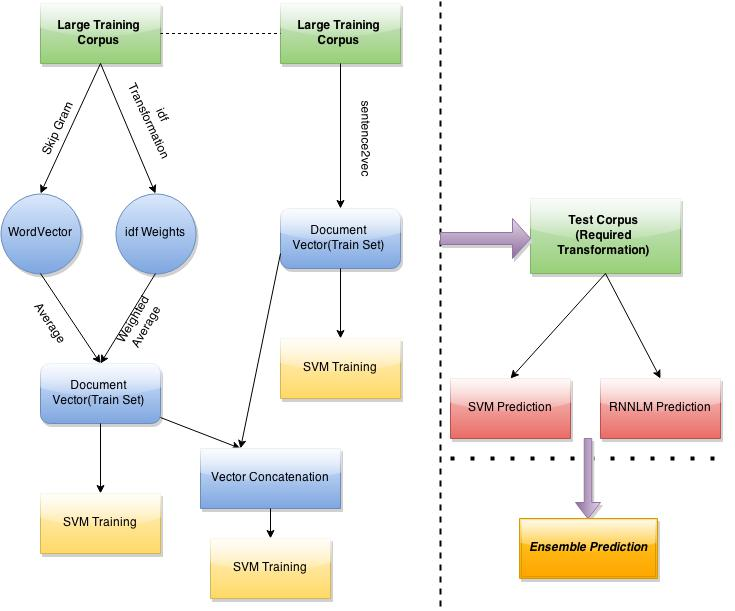
\includegraphics[scale=0.3]{../img/flow_chart.jpg}
	\caption{Work Flow}
	\label{fig:workflow}
    \end{figure}
}

%===========================================================================
\section[Results]{Results}
\subsection{}


%===========================================================================
\section[Conclusion and Future Work]{Conclusion and Future Work}
\subsection{}

%-------------------------------------slide---------------------------------
\frame{\frametitle{Weightages}
	\begin{block}{Song Features}
	\begin{itemize}
		\item Artist similarity has been assigned a weight of 60\%
		\item 20\% each for loudness \& tempo
		\item These values have been evaluated to good results
	\end{itemize}
  \end{block}
\pause
	\begin{block}{Similarity v/s Popularity}
	\begin{itemize}
		\item 65\% weightage has been assgined to similarity and 35\% to popularity
		\item A few number of test runs suggested the above weightages to be good
	\end{itemize}
	\end{block}
}
%-------------------------------------slide---------------------------------
\frame{\frametitle{Performance Evaluation}
  \begin{beamerboxesrounded}[shadow=true]{}
	\begin{itemize}
		 \item Most recent \emph{t} tracks have been considered for testing
		 \item Following \emph{m} tracks are taken for current mood
		 \item Recommended songs are then matched with the \emph{t} tracks
		 \item The rank of the top recommendation that appears in the test set is noted
		 \item The similarity of the most similar mood window is also noted
	\end{itemize}
  \end{beamerboxesrounded}
}
%-------------------------------------slide---------------------------------
\frame{\frametitle{Test Run 1}
  \begin{beamerboxesrounded}[shadow=true]{}
    \begin{table}[h!]
\centering
\begin{tabular}{ | c | c | c || c | c | }
\hline
Similar Users	& Mood Length	& Weights							&Confidence	&Rank\\
\hline \hline
50			& 5			& \(\rfrac{1}{3}, \rfrac{1}{3}, \rfrac{1}{3}\)	&62.89 \%		&944\\
\hline
75			& 5			& \(\rfrac{1}{3}, \rfrac{1}{3}, \rfrac{1}{3}\)	&48.45 \%		&3879\\
\hline
100			& 5			& \(\rfrac{1}{3}, \rfrac{1}{3}, \rfrac{1}{3}\)	&48.45 \%		&84\\
\hline
150			& 5			& \(\rfrac{1}{3}, \rfrac{1}{3}, \rfrac{1}{3}\)	&51.01 \%		&135\\
\hline
200			& 5			& \(\rfrac{1}{3}, \rfrac{1}{3}, \rfrac{1}{3}\)	&52.63 \%		&211\\
\hline
50			& 10			& \(\rfrac{1}{3}, \rfrac{1}{3}, \rfrac{1}{3}\)	&45.06 \%		&3418\\
\hline
75			& 10			& \(\rfrac{1}{3}, \rfrac{1}{3}, \rfrac{1}{3}\)	&45.50 \%		&4751\\
\hline
100			& 10			& \(\rfrac{1}{3}, \rfrac{1}{3}, \rfrac{1}{3}\)	&46.93 \%		&1722\\
\hline
50			& 5			& \(\rfrac{1}{5}, \rfrac{2}{5}, \rfrac{2}{5}\)	&43.28 \%		&4033\\
\hline
50			& 5			& \(\rfrac{3}{5}, \rfrac{1}{5}, \rfrac{1}{5}\)	&70.57 \%		&936\\
\hline
75			& 5			& \(\rfrac{3}{5}, \rfrac{1}{5}, \rfrac{1}{5}\)	&60.03 \%		&4367\\
\hline
100			& 5			& \(\rfrac{3}{5}, \rfrac{1}{5}, \rfrac{1}{5}\)	&62.10 \%		&78\\
\hline
150			& 5			& \(\rfrac{3}{5}, \rfrac{1}{5}, \rfrac{1}{5}\)	&64.73 \%		&120\\
\hline
\end{tabular}
\caption{Test Results for Last.FM user: \emph{3en}}
\label{table:test_results_3en}
\end{table}
  \end{beamerboxesrounded}
}
%-------------------------------------slide---------------------------------
\frame{\frametitle{Test Run 2}
  \begin{beamerboxesrounded}[shadow=true]{}
   \begin{table}[h!]
\centering
\begin{tabular}{ | c | c | c || c | c | }
\hline
Similar Users	& Mood Length	& Weights							&Confidence	&Rank\\
\hline \hline
50			& 5			& \(\rfrac{1}{3}, \rfrac{1}{3}, \rfrac{1}{3}\)	&62.39 \%		&2376\\
\hline
75			& 5			& \(\rfrac{1}{3}, \rfrac{1}{3}, \rfrac{1}{3}\)	&50.43 \%		&N/A\\
\hline
100			& 5			& \(\rfrac{1}{3}, \rfrac{1}{3}, \rfrac{1}{3}\)	&50.43 \%		&7608\\
\hline
150			& 5			& \(\rfrac{1}{3}, \rfrac{1}{3}, \rfrac{1}{3}\)	&50.43 \%		&8828\\
\hline
200			& 5			& \(\rfrac{1}{3}, \rfrac{1}{3}, \rfrac{1}{3}\)	&52.40 \%		&10018\\
\hline
50			& 10			& \(\rfrac{1}{3}, \rfrac{1}{3}, \rfrac{1}{3}\)	&48.91 \%		&N/A\\
\hline
75			& 10			& \(\rfrac{1}{3}, \rfrac{1}{3}, \rfrac{1}{3}\)	&48.91 \%		&N/A\\
\hline
100			& 10			& \(\rfrac{1}{3}, \rfrac{1}{3}, \rfrac{1}{3}\)	&48.91 \%		&N/A\\
\hline
50			& 5			& \(\rfrac{1}{5}, \rfrac{2}{5}, \rfrac{2}{5}\)	&43.28 \%		&N/A\\
\hline
50			& 5			& \(\rfrac{3}{5}, \rfrac{1}{5}, \rfrac{1}{5}\)	&70.70 \%		&2391\\
\hline
75			& 5			& \(\rfrac{3}{5}, \rfrac{1}{5}, \rfrac{1}{5}\)	&66.15 \%		&N/A\\
\hline
100			& 5			& \(\rfrac{3}{5}, \rfrac{1}{5}, \rfrac{1}{5}\)	&66.15 \%		&7095\\
\hline
150			& 5			& \(\rfrac{3}{5}, \rfrac{1}{5}, \rfrac{1}{5}\)	&66.15 \%		&7767\\
\hline
\end{tabular}
\caption{Test Results for Last.FM user: \emph{RJ}}
\label{table:test_results_rj}
\end{table}
  \end{beamerboxesrounded}
}
%-------------------------------------slide---------------------------------
\frame{\frametitle{Test Run 3}
  \begin{beamerboxesrounded}[shadow=true]{}
  \begin{table}[h!]
\centering
\begin{tabular}{ | c | c | c || c | c | }
\hline
Similar Users	& Mood Length	& Weights							&Confidence	&Rank\\
\hline \hline
50			& 5			& \(\rfrac{1}{3}, \rfrac{1}{3}, \rfrac{1}{3}\)	&62.59 \%		&59\\
\hline
75			& 5			& \(\rfrac{1}{3}, \rfrac{1}{3}, \rfrac{1}{3}\)	&50.43 \%		&607\\
\hline
100			& 5			& \(\rfrac{1}{3}, \rfrac{1}{3}, \rfrac{1}{3}\)	&48.37 \%		&736\\
\hline
150			& 5			& \(\rfrac{1}{3}, \rfrac{1}{3}, \rfrac{1}{3}\)	&51.94 \%		&1095\\
\hline
200			& 5			& \(\rfrac{1}{3}, \rfrac{1}{3}, \rfrac{1}{3}\)	&51.94 \%		&1428\\
\hline
50			& 10			& \(\rfrac{1}{3}, \rfrac{1}{3}, \rfrac{1}{3}\)	&48.91 \%		&2632\\
\hline
75			& 10			& \(\rfrac{1}{3}, \rfrac{1}{3}, \rfrac{1}{3}\)	&48.91 \%		&3736\\
\hline
100			& 10			& \(\rfrac{1}{3}, \rfrac{1}{3}, \rfrac{1}{3}\)	&46.91 \%		&4304\\
\hline
50			& 5			& \(\rfrac{1}{5}, \rfrac{2}{5}, \rfrac{2}{5}\)	&43.28 \%		&563\\
\hline
50			& 5			& \(\rfrac{3}{5}, \rfrac{1}{5}, \rfrac{1}{5}\)	&70.94 \%		&85\\
\hline
75			& 5			& \(\rfrac{3}{5}, \rfrac{1}{5}, \rfrac{1}{5}\)	&66.15 \%		&555\\
\hline
100			& 5			& \(\rfrac{3}{5}, \rfrac{1}{5}, \rfrac{1}{5}\)	&63.88 \%		&650\\
\hline
150			& 5			& \(\rfrac{3}{5}, \rfrac{1}{5}, \rfrac{1}{5}\)	&64.59 \%		&970\\
\hline
\end{tabular}
\caption{Test Results for Last.FM user: \emph{eartle}}
\label{table:test_results_eartle}
\end{table}
  \end{beamerboxesrounded}
}
%-------------------------------------slide---------------------------------
\frame{\frametitle{Test Run 4}
  \begin{beamerboxesrounded}[shadow=true]{}
  \begin{table}[h!]
\centering
\begin{tabular}{ | c | c | c || c | c | }
\hline
Similar Users	& Mood Length	& Weights							&Confidence	&Rank\\
\hline \hline
50			& 5			& \(\rfrac{1}{3}, \rfrac{1}{3}, \rfrac{1}{3}\)	&61.84 \%		&141\\
\hline
75			& 5			& \(\rfrac{1}{3}, \rfrac{1}{3}, \rfrac{1}{3}\)	&49.83 \%		&629\\
\hline
100			& 5			& \(\rfrac{1}{3}, \rfrac{1}{3}, \rfrac{1}{3}\)	&49.71 \%		&674\\
\hline
150			& 5			& \(\rfrac{1}{3}, \rfrac{1}{3}, \rfrac{1}{3}\)	&51.10 \%		&4351\\
\hline
200			& 5			& \(\rfrac{1}{3}, \rfrac{1}{3}, \rfrac{1}{3}\)	&51.48 \%		&4363\\
\hline
50			& 10			& \(\rfrac{1}{3}, \rfrac{1}{3}, \rfrac{1}{3}\)	&47.49 \%		&3160\\
\hline
75			& 10			& \(\rfrac{1}{3}, \rfrac{1}{3}, \rfrac{1}{3}\)	&47.49 \%		&3135\\
\hline
100			& 10			& \(\rfrac{1}{3}, \rfrac{1}{3}, \rfrac{1}{3}\)	&47.54 \%		&3225\\
\hline
50			& 5			& \(\rfrac{1}{5}, \rfrac{2}{5}, \rfrac{2}{5}\)	&43.28 \%		&4422\\
\hline
50			& 5			& \(\rfrac{3}{5}, \rfrac{1}{5}, \rfrac{1}{5}\)	&67.74 \%		&103\\
\hline
75			& 5			& \(\rfrac{3}{5}, \rfrac{1}{5}, \rfrac{1}{5}\)	&66.18 \%		&470\\
\hline
100			& 5			& \(\rfrac{3}{5}, \rfrac{1}{5}, \rfrac{1}{5}\)	&64.43 \%		&471\\
\hline
150			& 5			& \(\rfrac{3}{5}, \rfrac{1}{5}, \rfrac{1}{5}\)	&64.43 \%		&5227\\
\hline
\end{tabular}
\caption{Test Results for Last.FM user: \emph{franhale}}
\label{table:test_results_franhale}
\end{table}
  \end{beamerboxesrounded}
}
%-------------------------------------slide---------------------------------
\frame{\frametitle{Test Run 5}
  \begin{beamerboxesrounded}[shadow=true]{}
  \begin{table}[h!]
\centering
\begin{tabular}{ | c | c | c || c | c | }
\hline
Similar Users	& Mood Length	& Weights							&Confidence	&Rank\\
\hline \hline
50			& 5			& \(\rfrac{1}{3}, \rfrac{1}{3}, \rfrac{1}{3}\)	&62.64 \%		&4953\\
\hline
75			& 5			& \(\rfrac{1}{3}, \rfrac{1}{3}, \rfrac{1}{3}\)	&50.09 \%		&9857\\
\hline
100			& 5			& \(\rfrac{1}{3}, \rfrac{1}{3}, \rfrac{1}{3}\)	&50.09 \%		&11647\\
\hline
150			& 5			& \(\rfrac{1}{3}, \rfrac{1}{3}, \rfrac{1}{3}\)	&51.10 \%		&6587\\
\hline
200			& 5			& \(\rfrac{1}{3}, \rfrac{1}{3}, \rfrac{1}{3}\)	&51.48 \%		&8008\\
\hline
50			& 10			& \(\rfrac{1}{3}, \rfrac{1}{3}, \rfrac{1}{3}\)	&48.08 \%		&N/A\\
\hline
75			& 10			& \(\rfrac{1}{3}, \rfrac{1}{3}, \rfrac{1}{3}\)	&48.08 \%		&2584\\
\hline
100			& 10			& \(\rfrac{1}{3}, \rfrac{1}{3}, \rfrac{1}{3}\)	&48.08 \%		&2887\\
\hline
50			& 5			& \(\rfrac{1}{5}, \rfrac{2}{5}, \rfrac{2}{5}\)	&43.28 \%		&N/A\\
\hline
50			& 5			& \(\rfrac{3}{5}, \rfrac{1}{5}, \rfrac{1}{5}\)	&70.75 \%		&5005\\
\hline
75			& 5			& \(\rfrac{3}{5}, \rfrac{1}{5}, \rfrac{1}{5}\)	&65.97 \%		&7819\\
\hline
100			& 5			& \(\rfrac{3}{5}, \rfrac{1}{5}, \rfrac{1}{5}\)	&65.97 \%		&9345\\
\hline
150			& 5			& \(\rfrac{3}{5}, \rfrac{1}{5}, \rfrac{1}{5}\)	&68.19 \%		&5749\\
\hline
\end{tabular}
\caption{Test Results for Last.FM user: \emph{massdosage}}
\label{table:test_results_massdosage}
\end{table}
  \end{beamerboxesrounded}
}
%-------------------------------------slide---------------------------------
\frame{\frametitle{Optimizations}
  \begin{beamerboxesrounded}[shadow=true]{}
     \begin{itemize}
      \item Parallelization: Independent jobs have been forked in parallel to reduce runtime
      \item On-Demand Caching: Not only avoids loading the entire DB into memory, but also prevents disk access each time the same resource is called for. Also reduces multiple file accesses
      \item Minimal data handling: Minimal data is stored in memory in a serialized JSON format
     \end{itemize}
  \end{beamerboxesrounded}
}
%-------------------------------------slide---------------------------------
\frame{\frametitle{Future Work}
  \begin{beamerboxesrounded}[shadow=true]{}
	\begin{itemize}
		 \item Larger and newer dataset
		 \item Machine learning to implement feedback mechanism for user specific weightages
		 \item More features like MFCC can be included appropriately
		 \item Code can be optimized even further by the use of distributed systems
	\end{itemize}
  \end{beamerboxesrounded}
}

%-------------------------------------slide---------------------------------
\frame{\frametitle{}
%  \begin{beamerboxesrounded}[shadow=true]{}
   %\centering{\Large{Questions?}}
    \begin{figure}
      \centering
      
\includegraphics[scale=0.2]{../img/questions.png}
    \end{figure}
%  \end{beamerboxesrounded}
}

%-------------------------------------slide---------------------------------
\frame{\frametitle{}
  \begin{beamerboxesrounded}[shadow=true]{}
   \centering{\Large{Thank you!}}
  \end{beamerboxesrounded}
}
\end{document}
